\documentclass{llncs}

\usepackage[english]{babel}
\usepackage[tight]{subfigure}
% \usepackage{floatrow}
\usepackage{epsfig}
\usepackage{amsmath}

\begin{document}

\title{A simple shell model for real-time simulation of intra-ocular implant deployment}
\author{Olivier Comas, St\'ephane Cotin and Christian Duriez}
\institute{INRIA, Alcove team, Lille, France}

\maketitle

\begin{abstract}
With 30 million interventions a year worldwide, cataract surgery is one of the most frequently performed procedures. Yet, no tool currently allows teaching all steps of the procedure without putting patients at risk. A particularly challenging stage of this surgery deals with the injection and deployment of the intraocular lens implant. In this paper we propose to rely on thin plate theory to accurately describe the large bending of the implant. Our approach extends the co-rotational method used in finite element analysis to incorporate a bending energy. This results in a relatively simple and computationally efficient approach which was applied to the simulation of the lens' deployment. This simulation also accounts for the complex contacts that take place between the implant and the injection device. Particular care was given to the validation of the proposed model as well as its stability. 
\end{abstract}

\section{Introduction}
According to the latest assessment of the World Health Organization, age related cataract is responsible for $48\,\%$ of world blindness, which represents about 18 million people. Cataract is the clouding of the lens of the eye which impedes the passage of light. Its treatment is a surgical operation, which is very successful in restoring sight. The opaque lens is removed and replaced by an artificial intraocular lens. As people in the world live longer, the number of people with cataract is growing.  Current methods of teaching based on companionship not only expose patient to complications inherent to the inexperience of the operator, but they are also not very adequate with the increasing demands in training for this procedure. The development of a cataract surgery simulator could offer a new way of learning for young ophthalmologists. This work focuses on intraocular lens modelling to simulate the crucial step of the surgery dealing with the lens injection and its deployment within the lens capsule. 

The implant is a three-dimensional structure, thin in one direction and long in the other two directions and may be characterised as a thin object. Thin objects are usually classified in two categories: plates and shells. The difference between these two kinds of structure is very well explained by Liu \cite{Liu03}. A plate structure carries only transversal loads that lead to bending deformation. As an example, consider the horizontal boards of a bookshelf that supports books. Those boards can be approximated as a plate structure and the transversal loads are of course the weight of the books. Conversely, a shell structure carries loads in all directions, and therefore undergoes bending, twisting and in-plane deformation, like the fuselage of an aircraft. Considering the folded position of the implant within the injection device (figure \ref{fig-surgery}), we need to model the intraocular implant as a shell. 
% + 2 EXAMPLES TO ILLUSTRATE THE DIFFERENCE BETWEEN PLATE AND SHELL

%\begin{figure}[h]
%\begin{center}
%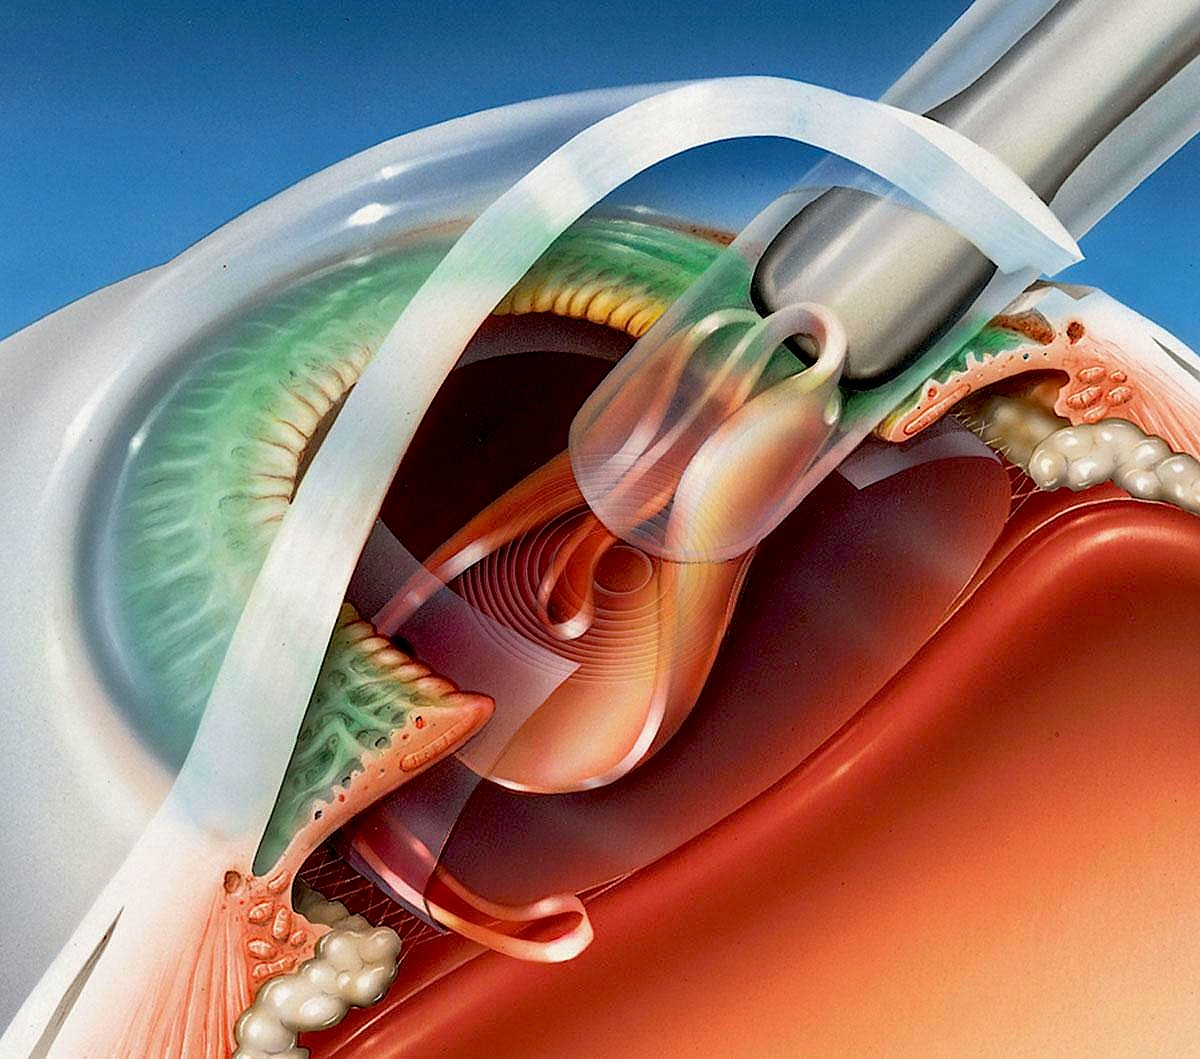
\includegraphics[width=6cm]{images/deployment}
%\caption [Implant within injector] {Insertion of the lens implant through the injector}
%\label{fig-injector}
%\end{center}
%\end{figure}

\subsection{Related work}

Numerous models are available in the literature to describe physics of thin objects, from fairly simple and naive approaches to more complex and thourought representations. Continuum mechanics provides many formulations able to accurately describe stresses occuring within thin objects, all of them fall into two categories depending whether they are based on plate or shell theory. Those theories have been a subject of interest in the mechanical community for decades. Plate theory can be inferred from shell theory by considering the special case of planar midsurfaces \cite{Chapelle03}. Indeed it is often not necessary to use three-dimensional elasticity theory like in shell theory to model plates. Simple two-dimensional theories that account for bending deformation of thin bodies have been developped, and they are known as plate theories \cite{Reddy05}. However, formulations based on continuum mechanics are often quite complex and they are not always suitable for real-time applications. Therefore many researchers have tried to circumvent this limit. One of the most successful approach is the mass-spring model \cite{Provot95,Hammer08,Yu08}. Not only elasticity parameters included in mass-springs systems have no relation with the physical parameters but this type of model does not account for bending. Another type of modelling is position based approaches, which rely on projection as a complete simulation method \cite{Muller07}. Those approaches use impulses instead of forces to control the animation. Because impulses directly change velocities, one level of integration can be skipped. While this is an interesting approach for computer game industry, the main drawback of this method is that it is not physically accurate. So is the approach of Grinspun \emph{et al.} \cite{Grinspun03}, targeted at computer animation, which geometrically derives a discrete model for thin shells. Finite difference method \cite{Terzopoulos87} and finite element method have also been widely used, especially in cloth modelling, which is a very active field in computer graphics \cite{Volino00}. 
% TOO MANY REFERENCES OUTSIDE SHELLS?

\subsection{Our approach}

Our idea is to create a shell element by combining a classic two-dimensional element to handle the in-plane forces (membrane) and a plate element for off-plane forces (bending and twisting). However our real-time requirements demands a computationally inexpensive formulation and we would like to introduce the co-rotational framework to thin plate theory. Indeed co-rotational approaches have been successfully applied to real-time simulation of volumetric objects by the community over the last few years. They offer a good trade-off between computational efficiency and accuracy by allowing materially linear FEM to handle large deformations. We propose to improve and extend a plate model first introduced by Przemieniecki \cite{Przemieniecki68} to a co-rotational formulation. Once combined with a two-dimensional formulation, we obtain an accurate, yet computationally efficient, shell finite element method featuring both membrane and bending energies. 


\section{Plate model's description}

\subsection{Triangular elastic membrane}
The computation of the triangular elastic membrane stiffness matrix can be simply derived from previous works dealing with tetrahedral co-rotational elements (see Muller \emph{et al.} \cite{Muller04}) for instance. The element stiffness matrix $\textbf{K}_e$ can be computed as follows:

\begin{equation}
\textbf{K}_e = \int_v \textbf{J} \boldsymbol\chi \textbf{J}^{T} dV
\end{equation} 

where $\textbf{J}$ is the strain-displacement matrix and $\boldsymbol\chi$ embodies the material's behaviour. In the simple case of Hooke's law we have:

\begin{equation}
\boldsymbol\chi = \frac{E}{12(1-\nu^2)}
	\begin{bmatrix}
	1 & \nu & 0 \\
 	\nu & 1 & 0 \\
	0 & 0 & \frac{1}{2} (1-\nu)
	\end{bmatrix}
\end{equation} 

The stiffness matrix in the global frame is eventually obtained using the rotation matrix of the element: $\textbf{K} = \textbf{R} \textbf{K}_e \textbf{R}^{T}$.

\subsection{Thin plate theory}

Since the computation of the membrane stiffness matrix is classic and presents no difficulty, we will only detail the bending part of the formulation. To calculate the stiffness matrix for the transverse deflections and rotations shown on figure \ref{fig-triangle}, we start with the assumed deflection $u_z$ of the form

\begin{equation}
 u_z = c_1 + c_2x + c_3y + c_4x^2 + c_5xy + c_6y^2 + c_7x^3 + c_8xy^2 + c_9y^3
\label{eq-deflection}
\end{equation} 

where $c_1$, \ldots , $c_9$ are constants. An issue of symmetry was observed with the deflection proposed by Przemieniecki, but was corrected by removing the term $x^2y$ in factor of the 8th constant. These constants can be evaluated in terms of the displacements and slopes at the three corners of the triangular plate using 
\begin{equation}
\textbf{u} = \textbf{Cc}
\label{eq-U}
\end{equation} 
where $\textbf{u} = \left\{u_1 u_2 \ldots u_9 \right\} $ and $\textbf{c} = \left\{c_1 c_2 \ldots c_9 \right\} $ while the matrix $\textbf{C}$ is given by
\begin{equation}
C = 
	\begin{bmatrix}
	1 & 0 & 0 & 0 & 0 & 0 & 0 & 0 & 0 \\
 	0 & 0 & 1 & 0 & 0 & 0 & 0 & 0 & 0 \\
	0 & -1 & 0 & 0 & 0 & 0 & 0 & 0 & 0 \\
	1 & x_2 & 0 & x_2^2 & 0 & 0 & x_2^3 & 0 & 0 \\
	0 & 0 & 1 & 0 & x_2 & 0 & 0 & 0 & 0 \\
	0 & -1 & 0 & -2x_2 & 0 & 0 & -3x_2 & 0 & 0 \\
	1 & x_3 & y_3 & x_3^2 & x_3y_3 & y_3^2 & x_3^2 & x_3y_3^2& y_3^3 \\
	0 & 0 & 1 & 0 & x_3 & 2y_3 & 0 & 2x_3y_3 & 3y_3^2 \\
	0 & -1 & 0 & -2x_3 & -y_3 & 0 & -3x_3^2 & -y_3^2 & 0
	\end{bmatrix}
\end{equation} 
in deriving equation \ref{eq-U}. The notation 

\begin{equation}
(u_z)_{x_1,y_1} = u_1 \hspace{1cm} \left(\frac{\partial u_z}{\partial y}\right)_{x_1,y_1} = u_2 \hspace{1cm} \left(\frac{\partial u_z}{\partial x}\right)_{x_1,y_1} = -u_3
\end{equation} 
and so on, has been used.

\begin{figure}
\begin{center}
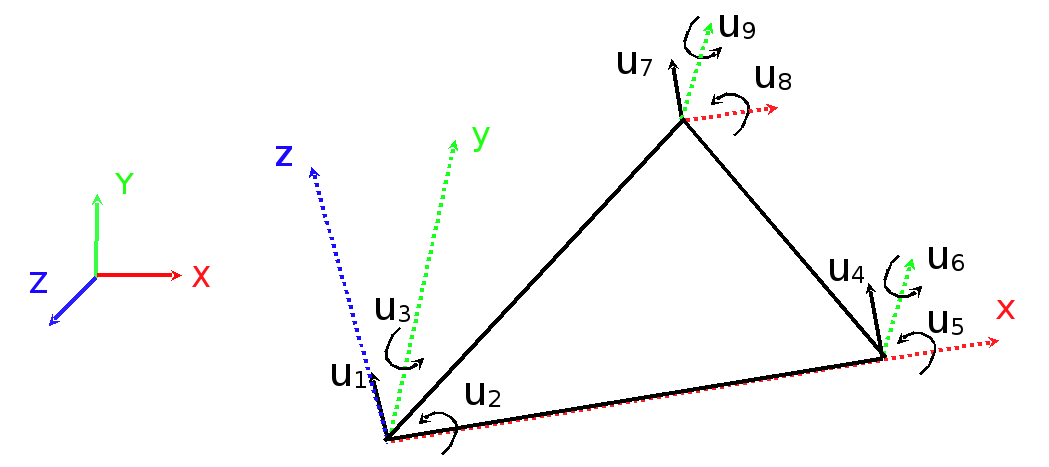
\includegraphics[width=12cm]{images/triangle}
\caption {Triangular plate element in bending}
\label{fig-triangle}
\end{center}
\end{figure}

We can calculate the strains from the flat-plate theory using
\begin{equation}
e_{xx} = -z \frac{\partial^2u_z}{\partial x^2}
\end{equation} 
\begin{equation}
e_{yy} = -z \frac{\partial^2u_z}{\partial y^2}
\end{equation} 
\begin{equation}
e_{xy} = -2z \frac{\partial^2u_z}{\partial x \partial y}
\end{equation} 
Hence, using the above equations and equation \ref{eq-deflection}, we have
\begin{equation}
\begin{bmatrix}
e_{xx} \\
e_{yy} \\
e_{xy}
\end{bmatrix}
= 
-z
\begin{bmatrix}
0 & 0 & 0 & 2 & 0 & 0 & 6x & 0 & 0 \\
0 & 0 & 0 & 0 & 0 & 2 & 0 & 2x & 6y \\
0 & 0 & 0 & 0 & 2 & 0 & 0 & 4y & 0 \\
\end{bmatrix}
\textbf{c}
\label{eq-strains}
\end{equation} 
or symbolically $\textbf{e} = \textbf{Dc}$ where $\textbf{D}$ stands for the $3\times 9$ matrix in equation \ref{eq-strains}, including the premultiplying constant $-z$. Noting from equation \ref{eq-U} that $\textbf{c} = \textbf{C}^{-1}\textbf{u}$, we have 
\begin{equation}
\textbf{e} = \textbf{DC}^{-1}\textbf{u} = \textbf{bu}
\end{equation} 
where $\textbf{b} = \textbf{DC}^{-1}$. 
Knowing that the stiffness matrix $\textbf{K}_e$ for an element is obtained from
\begin{equation}
\textbf{K}_e = \int_v \textbf{b}^{T} \boldsymbol\chi \textbf{b} dV
\end{equation} 
where $\boldsymbol\chi$ is the material matrix. The substitution of $\textbf{b}$ into this expression yields
\begin{equation}
\textbf{K}_e = (\textbf{C}^{-1})^T \int_v \textbf{D}^{T} \boldsymbol\chi \textbf{D} dV \textbf{C}^{-1}
\end{equation} 
The integration is carried out numerically using Gauss points located at the centre of each edge. 

\subsection{Implementation}

This plate formulation has been successfully implemented into the open-source framework SOFA \cite{SOFA}. In practice the formulation is very simple and for each triangle it consists of the following steps:

\begin{enumerate}
\item compute the rotation matrix from global to triangle (local) frame
\item measure the orientation of each vertex in the local frame and compare it to the local orientation obtained for the rest position to compute the local displacement vector $\textbf{u} = \left\{0 \, \Omega _{Ax} \, \Omega _{Ay}  \hspace{0.5cm} 0 \, \Omega _{Bx} \, \Omega _{By}  \hspace{0.5cm}  0 \, \Omega _{Cx} \, \Omega _{Cy} \right\}$. Indeed in a co-rotational framework the normal displacement of each vertex is locally null and only the rotation around the local $x$ and $y$ axes need to be measured at each of the three vertices A, B and C.
\item the matrix $\textbf{D}_i$ is expressed at each Gauss point $i$
\item the strain-displacement matrix at each Gauss point $i$ is calculated with $\textbf{J}_i = \textbf{D}_i \textbf{C}^{-1}$
\item the local stiffness matrix of the element $\textbf{K}_e$ is then obtained $\textbf{K}_e = \displaystyle{\sum^3_{i=1}} \textbf{J}_i \boldsymbol\chi \textbf{J}_i^T$
\item if a direct solver is used, the local element stiffness matrix is transformed into the global frame and added to the global stiffness matrix
\end{enumerate}

\section{Validation}

We compared the model with some theoretical results to assess its quality in modelling bending. The test that we carried out uses a square shape mesh clamped on the edges. A uniform pressure is then applied on the square and the maximum deflection $z_{max}$ at the centre can be calculated. In his paper Zhongnian \cite{Zhongnian86} uses the following parameters:
\begin{itemize}
 \item Young Modulus $E = 1.092 \times 10^6$
 \item Poisson's ratio $\nu = 0.3$
 \item edge of the square $L = 10\,m$
 \item thickness $h = 0.1\,m$
 \item pressure q is a uniformly distributed load per unit area
\end{itemize}

It can be shown that $z_{max} = 0.126\,q$. We experimentally measured the maximum deflection for different values of pressure $q$ (see table \ref{tab-results}). In average we found $z_{max} = 0.1248\,q $. Hence a $0.93\,\%$ error between our model and the theory on that test.

\begin{table}[h!]
	\begin{center}
		\begin{tabular}{|p{1.7cm}|p{1.7cm}|p{1.7cm}|p{1.7cm}|p{1.7cm}|p{1.7cm}|}
		\hline
		 \centering q & \centering 1 & \centering 2 & \centering 3 & \centering 4 & \centering 5 \tabularnewline
		\hline
		\centering $z_{max}$ & \centering 0.1218 & \centering 0.2475 & \centering 0.3747 & \centering 0.505 & \centering 0.637 \tabularnewline
		\hline
		\end{tabular}
	\vspace{0.3cm}
	\caption{Experimental results}
	\label{tab-results}
	\end{center}
\end{table}

\section{Injection and deployment of the intraocular implant}
\subsection{Description of cataract surgery procedure}
Cataract surgery is the removal of the natural lens of the eye (also called \emph{crystalline lens}) that has developed an opacification, which is referred to as a cataract. Metabolic changes of the crystalline lens fibers over the time lead to the development of the cataract and loss of transparency, causing impairment or loss of vision. During cataract surgery, a patient's cloudy natural lens is removed and replaced with a synthetic lens to restore the lens' transparency (figure \ref{fig-surgery}). The last step in the simulation of this surgery is the injection of the implant and its deployment within the lens capsule.

\begin{figure}[h]
\begin{center}
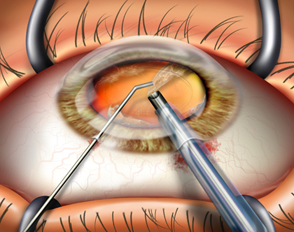
\includegraphics[height=4.5cm]{images/suction}
\hspace{0.2cm}
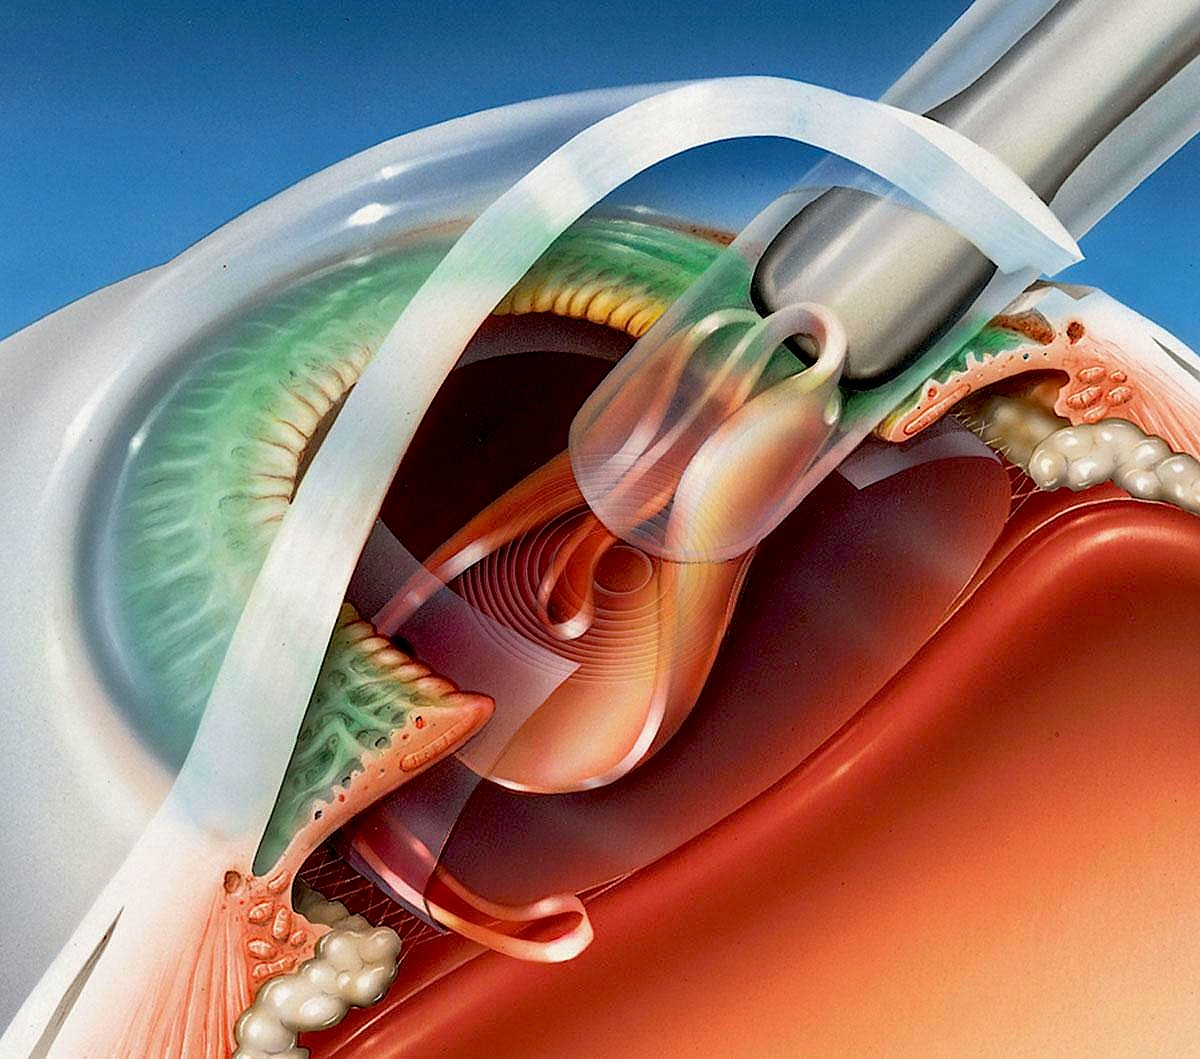
\includegraphics[height=4.5cm]{images/deployment}
\caption [Cataract surgery] {Left: removal of the opacified lens. Right: insertion of the lens implant.}
\label{fig-surgery}
\end{center}
\end{figure}

% Ref suction : http://www.coastal-eye-care-maine.com/cataracts-surgery/cataract-surgery-maine.html

%\begin{figure}[h]
%\begin{center}
%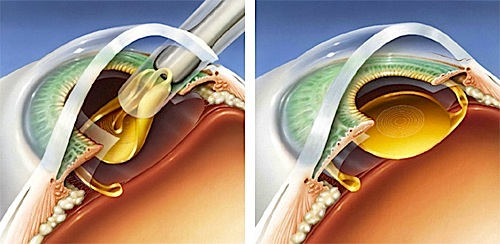
\includegraphics[height=4.5cm]{images/implant_injection}
%\caption [Cataract surgery] {Left: insertion of the lens implant. Right: deployment within the eye}
%\label{fig-surgery2}
%\end{center}
%\end{figure}


\subsection{Simulation}

A mesh of lens implant with the proper geometry has been designed with Blender (figure \ref{fig-implant}). The physical parameters have been provided by the manufacturer Alcon (table \ref{tab-parameters}). 

\begin{table}[h!]
	\begin{center}
		\begin{tabular}{|p{3cm}|p{3cm}|p{3cm}|}
		\hline
		 \centering Young's modulus & \centering Poisson's ratio & \centering Mass density \tabularnewline
		\hline
		\centering $1 MPa$ & \centering $0.42$ & \centering $1.2 g/cm^3$ \tabularnewline
		\hline
		\end{tabular}
	\vspace{0.3cm}
	\caption{Physical parameters of the intraocular implant (source: Alcon)}
	\label{tab-parameters}
	\end{center}
\end{table}

We start by folding the haptics onto the implant body, then the body is bent while keeping the haptics inside to obtain the same position as the one chosen by the surgeon when he puts the implant inside the injection device (figure \ref{fig-implantFolded}). The bent implant is then placed into the injection device. The simulation eventually consists of pushing the intraocular implant within the injection device into the eye. We can notice the progressive deployment of the implant when it slowly gets out of the injector. 
% + SCREENSHOTS OF SIMULATION

\begin{figure}[!h]
\begin{center}
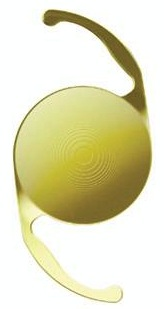
\includegraphics[height=6.5cm]{images/IOL}
\hspace{1cm}
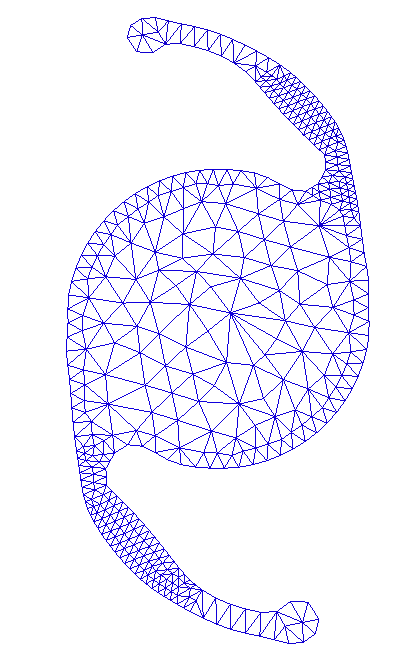
\includegraphics[height=6.5cm]{images/mesh_implant}
\caption [Lens implant and its mesh] {The real implant and the mesh created with Blender (473 triangles)}
\label{fig-implant}
\end{center}
\end{figure}

\begin{figure}[!h]
\begin{center}
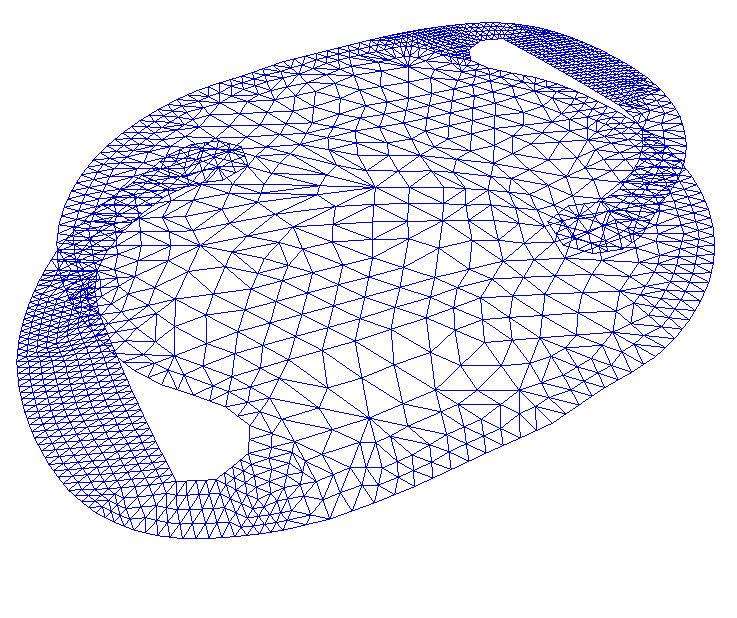
\includegraphics[height=5.5cm]{images/implant_haptics_in}

\includegraphics[height=5.5cm]{images/implant_folded}
\caption [Lens imlant] {Folding of the intraocular implant}
\label{fig-implantFolded}
\end{center}
\end{figure}

\section{Conclusion}

We improved a plate finite element formulation by extending it to a co-rotational framework in order to handle large deformations. By combining this formulation to a classic two-dimensional element we created a simple shell element able to efficiently handle both membrane and bending forces. The validity of our approach has been demonstrated though comparison with theoretical results and a non-trivial application in cataract surgery simulation.
% + NEXT STEPS

 \bibliographystyle{splncs}
 \bibliography{bibliography}


\end{document}